% LINGI2255 - Software Development Project
% Phase 2 - Architecture report
% Framework choice
\documentclass[11pt, a4paper]{article}   	% use "amsart" instead of "article" for AMSLaTeX format
\usepackage[utf8]{inputenc}
\usepackage[UKenglish]{babel}
\usepackage{graphicx}

\usepackage{amssymb}
\usepackage{xcolor}
\usepackage{hyperref}
\usepackage{url}
\usepackage{csquotes}
\usepackage{listings}
\lstset{language=Python}

\newcommand{\tbf}[1]{\textbf{#1}}
\newcommand{\tit}[1]{\textit{#1}}


\title{Brief Article}
\author{The Author}
%\date{}							% Activate to display a given date or no date

\begin{document}
%\maketitle

\section{Simulator}

We chose Selenium\footnote{\url{http://www.seleniumhq.org/}} to automate the testing of the web application.
An interesting feature is that we can actually see the actions performed in real time.

Selenium is composed of different components, but the one that we're interested in is the Selenium WebDriver\footnote{\url{http://www.seleniumhq.org/projects/webdriver/}}. % with the Selenium-Server
Its purpose is to drive a browser natively, either on a local or remote machine.
It gives the ability to send commands to a browser and to retrieve the results.
The Selenium WebDriver uses specific drivers to interact with browsers.
There are drivers for multiple browsers, including Chrome, Firefox and the Android browser.

\medskip
The tests can be written in multiple languages, including Java, Python and Ruby.
We chose to use Python because it is a simple, yet powerful language, and we will also use it for the web application.

\medskip
We don't know yet if it will be possible to deploy the simultor in grid to be able to stress our system.
But we will, at least, be able to run more than one instance to give us an idea of how the system performs in real conditions.


\section{Extension}

Our extension is social media.
It consists of allowing the users to login with a Facebook or Google account.
We decided to add the possibility to sign in with a Twitter account, because we think it could allow more users to easily use the web application.

\medskip
We will use the Django framework to build the web application, and it offers a built-in user authentication system.
It handles user accounts, groups, permissions and cookie-based user sessions. 
There are many packages available that can be installed to extend the possibilities of a Django project.
We searched for one that could help us for this task, and we chose to use the Django-Allauth\footnote{\url{https://www.djangopackages.com/packages/p/django-allauth/}} package to manage users authentication with Facebook, Google, or Twitter.
It is an interesting package because it supports a lot of authentication services, so that we could add more in the future if it is relevant.
Furthermore, it supports Python3 and Django 1.7, the latests stable versions.

\subsection*{How it will integrate with the system}
When the user sign in via a third-party provider, the module will create a \textit{user} object in the system as a standard registration.
The only difference is that this user will have no password associated.
Instead, another object \textit{Social account} will exists which will permit the user to sign in.
Since it is hard to automate registration and connection by third-party providers, we will not be able to test this extension via the simulator.


\section{User-Interface design}
The user interface has become increasingly important and complex.
Nowadays, UI frameworks are highly used by front-end developers.
Naturally, we looked for a UI framework that meets our needs.
\textit{Twitter Bootstrap} is a reference in this domain.
It encourage the use of responsive design, which means that the UI will adapt to the screen it is displayed on.
Furthermore, it promotes minimalist UI design that makes it is easier and quicker for the user to access information. This is why, we decided to use \textit{Twitter Bootstrap}.


\section{Sequence diagrams}

The sequence diagrams are based on the same use cases than the activity diagrams. In our first report, it lacked some details and we wanted
to compensate the deficiencies with sequence diagrams. In the second report, we also added the \enquote{create account} sequence diagram because we think that it is a important part of the user work-flow even if normally the user only register once.

In this report, we have modified some of the sequence diagrams and created a new one called \enquote{LoginWithSocialMedia} to take into account the remarks made after our second report about some inconsistencies and the social media extension.

You can see below the modified diagrams and their descriptions.

\begin{figure}[!ht]
   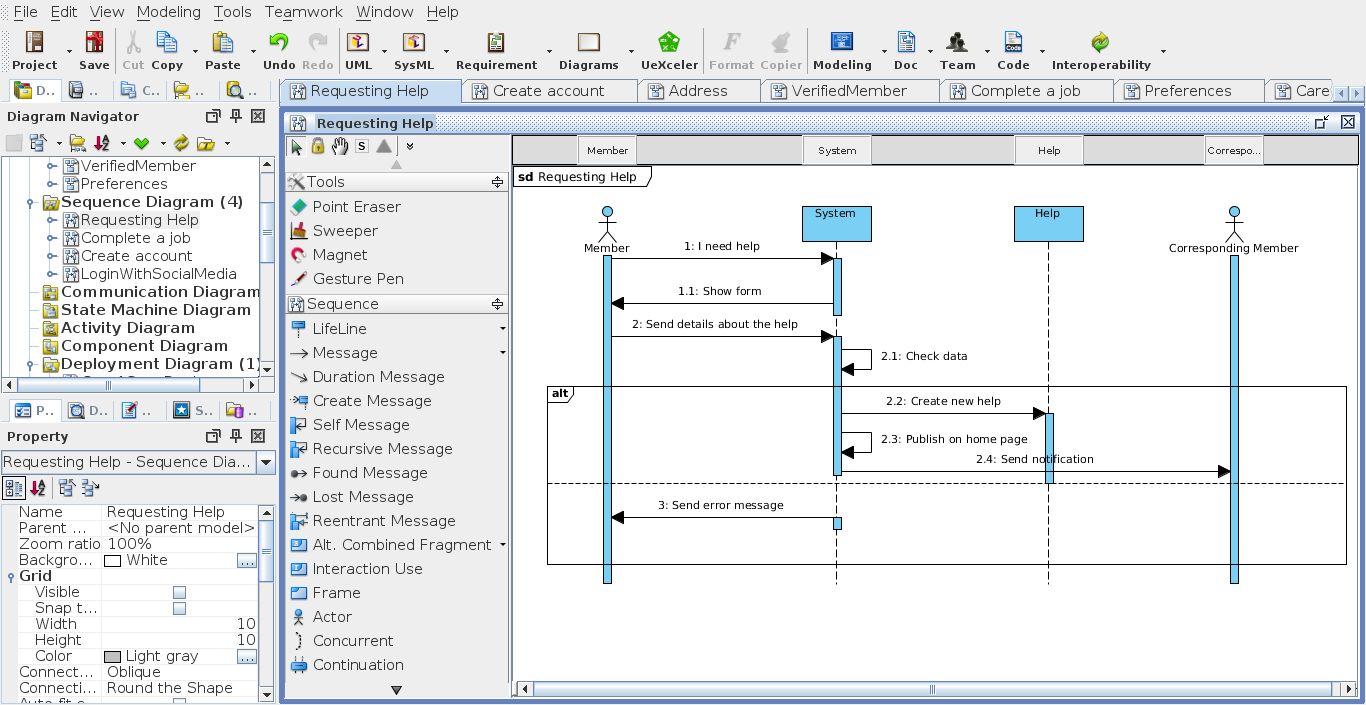
\includegraphics[width=\textwidth]{requestHelp.png}
   \caption{\label{requestHelp} Request Help}
\end{figure}

On figure ~\ref{requestHelp} : The user need some help and he is going to create a new request. For that he click on the \enquote{I need help}
and he is redirected to a page where he needs to fill in informations about the jobs. Afterward the system check the data entered by the user.
If it is correct create the request and add it to the list of request on the home page. The system also send a notification to the members that
correspond to the criteria of the request using their preferences. If the data are not correct it send an error message to the user.

The main modification on figure {requestingHelp} is that the action \enquote{publish on home page} is now done by the system. 

\begin{figure}[!ht]
   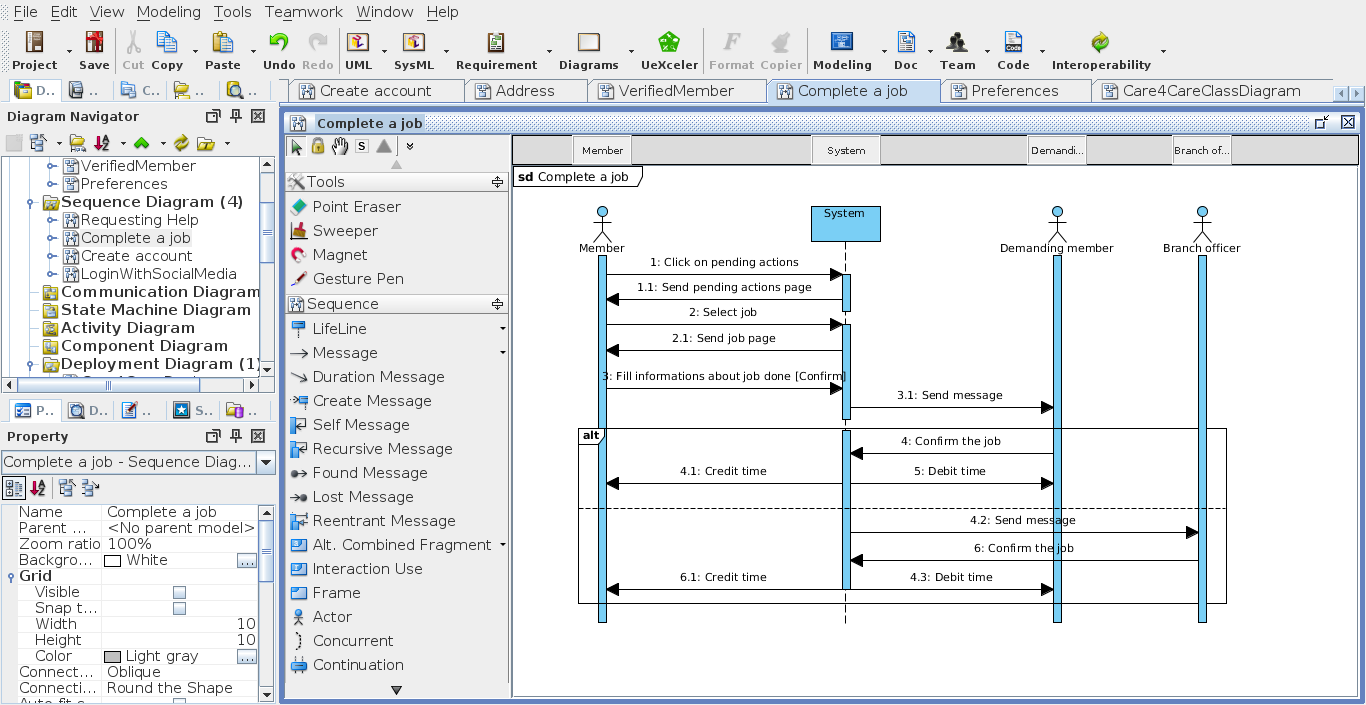
\includegraphics[width=\textwidth]{completeJob.png}
   \caption{\label{completeJob} Complete Job}
\end{figure}

On figure ~\ref{completeJob} : The user has completed a job and want to get time credit for it. For that he needs to go to the pending actions page (list all the jobs that the member accepted but did not completed yet) and select the corresponding job. He will then fill informations about the job and confirm. 

The system will send a notification to the demanding member (member which has been helped) and this member need to confirm that the job has been done correctly.

Unfortunately it can happen that the member does not confirm because for example, he has no Internet access. In this case, after some times, the system will send a message to the branch officer and ask him to confirm by himself.

The main modification on figure {completeAJob} is that the system send a message to the branch officer if the demanding member does not confirm after a certain period of time. (I didn't find a way to show the waiting time)

\subsection{Login with Social Media}

\begin{figure}[!ht]
   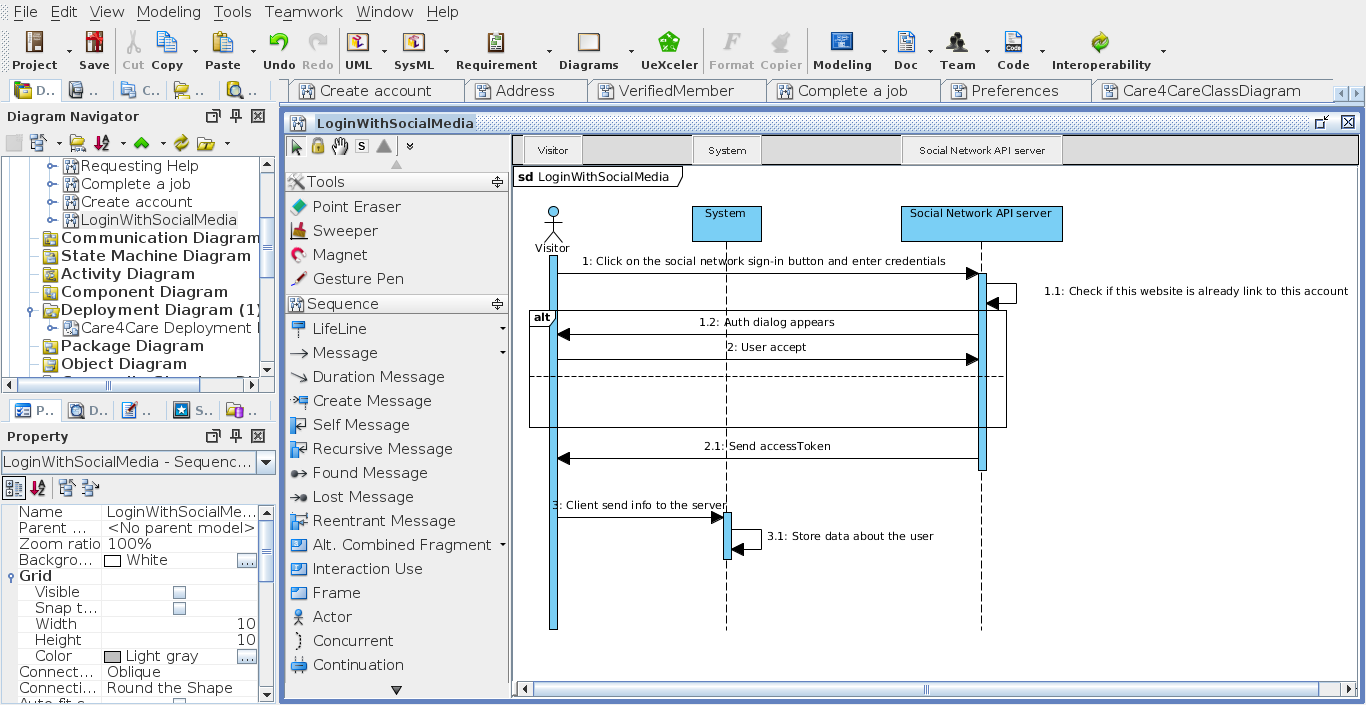
\includegraphics[width=\textwidth]{loginWithSocialMedia.png}
   \caption{\label{loginWithSocialMedia} Login with social media}
\end{figure}

On the figure ~\ref{loginWithSocialMedia} you can see that the client wants to authenticate using a social media like Google+ or Facebook. These social medias all give the possibility to sign in on your web site using their account. Usually they have multiple way to do it but the most common one is using Javascript that call a API. We choose that approach because we plan to support multiple social media.

In fact in this diagram the client directly contact the social media API server using Javascript to login. Than the social media API server check if the credential are correct and if the user already allowed this website to access his account and ask the user permission otherwise. 
Finally the server send back the token which will be use to authenticate the user for the API calls and the client will send some informations about his account to our application.


\section{Class diagrams}

About the main class diagram there was a few mistakes and some missing features about the social media extension. 

We tried to correct this by modifying our main class diagram and creating new small diagrams.


\subsection{Main class diagram}

\begin{figure}[!ht]
   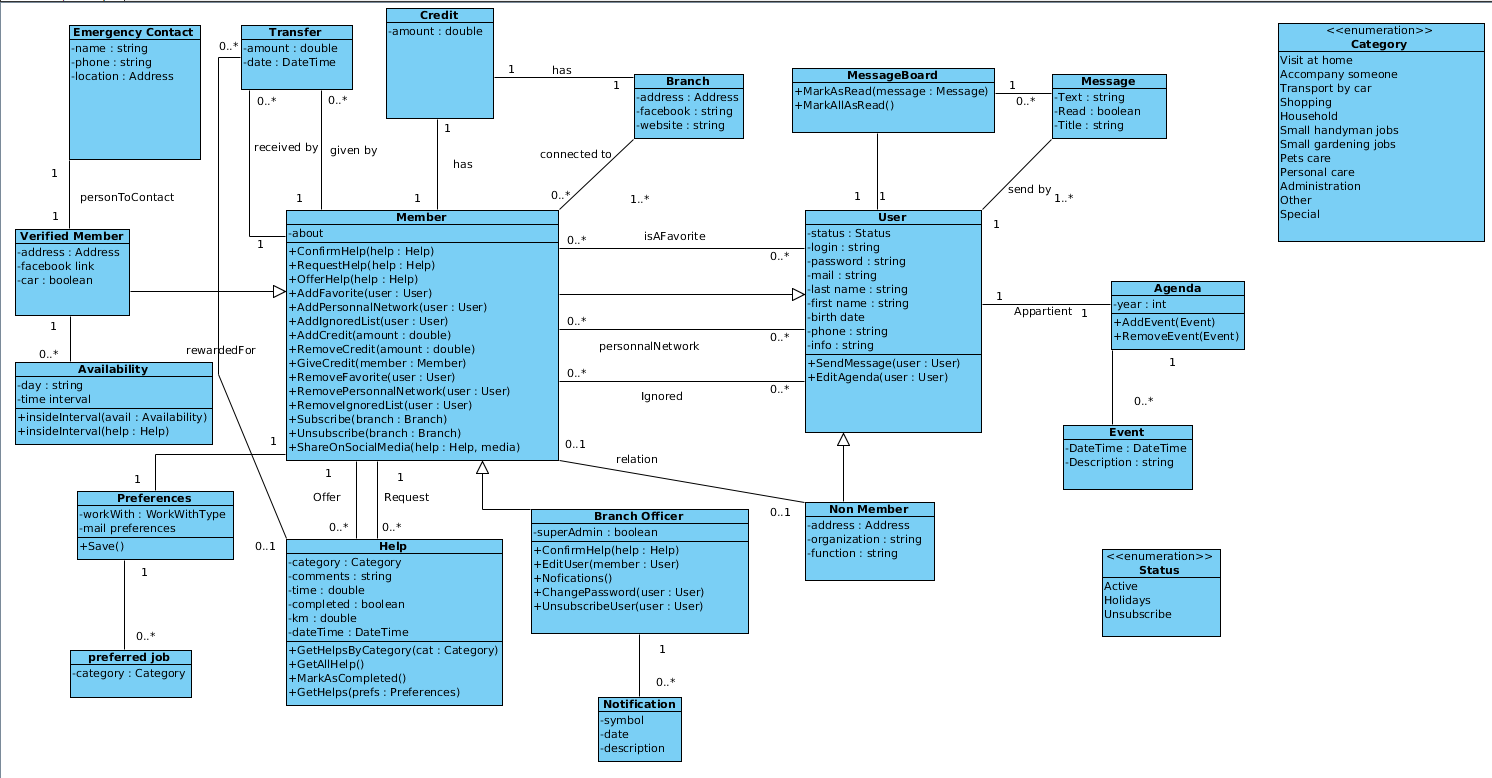
\includegraphics[width=\textwidth]{phase3MainClassDiagram.png}
   \caption{\label{phase3MainClassDiagram} Main class diagram}
\end{figure}


On the figure ~\ref{phase3MainClassDiagram},our main class diagram, we did the following changes :

\begin{itemize}
\item We added all the missing parameters to the function
\item We added new function to some classes 
\item We added type to attributes
\item We created new classes
\end{itemize}

\subsubsection{Transfer class}

The new classe Transfer will be use to track credit gifts from member and credit rewards for completed jobs. This class is link with two member, a giver and a receiver and optionally with a Help in case of a reward. This will enable us to keep a history of all the transactions of a user.

\subsubsection{Member class}

The class member has now more functionality :
\begin{itemize}
\item A function to share on a social Media like Facebook / Google+
\item Some functions to add/remove a user to/from their personal network/favorite/ignored list.
\item Some functions to (un)subscribe to a branch.
\end{itemize}

\subsubsection{Help class}

The class help has now function regarding searching for features and demands
\begin{itemize}
\item A function to get all the helps.
\item A function to get all the helps for a specific category.
\item A function to get all the helps depending on user preferences.
\end{itemize}

\subsection{Verified member diagram}

\begin{figure}[!ht]
   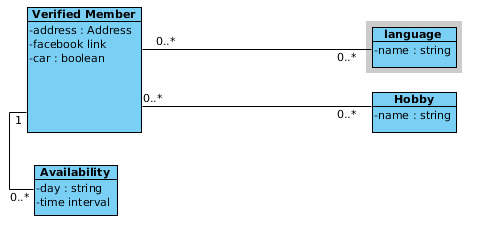
\includegraphics[width=\textwidth]{verifiedMember.png}
   \caption{\label{verifiedMember} Verified Member}
\end{figure}

On figure ~\ref{verifiedMember} you can see new class diagram which describe in more details the attributes of the class.

The time availability, language and hobby are now separate classes instead of attributes because they will be more complexe things to represent in our program. For example language and hobby are list of values and time availability is a object with method like \enquote{insideInterval} to check if some Help can be match with a user schedule.

\subsection{Preferences and Address diagrams}

\begin{figure}[!ht]
 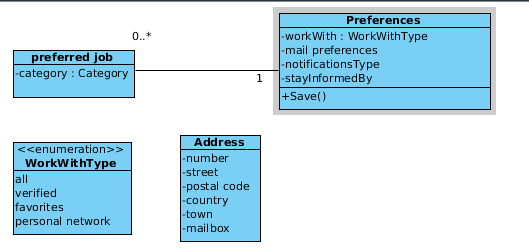
\includegraphics[width=\textwidth]{preferences.png}
   \caption{\label{preferences} Preferences and address diagrams}
\end{figure}

On figure ~\ref{preferences} we represented the class address that we didn't do last time. And we also went into more details
for the class preferences.



\section{Team Organization}

To do the job, we have divided our team into groups of two.
Then we divided the jobs in tasks that have been then assigned to groups.
We set some deadlines to avoid last minute rush.
To organize our work, we use several tools including Trello and Github. 

\subsection{Trello}

\begin{figure}[!ht]
   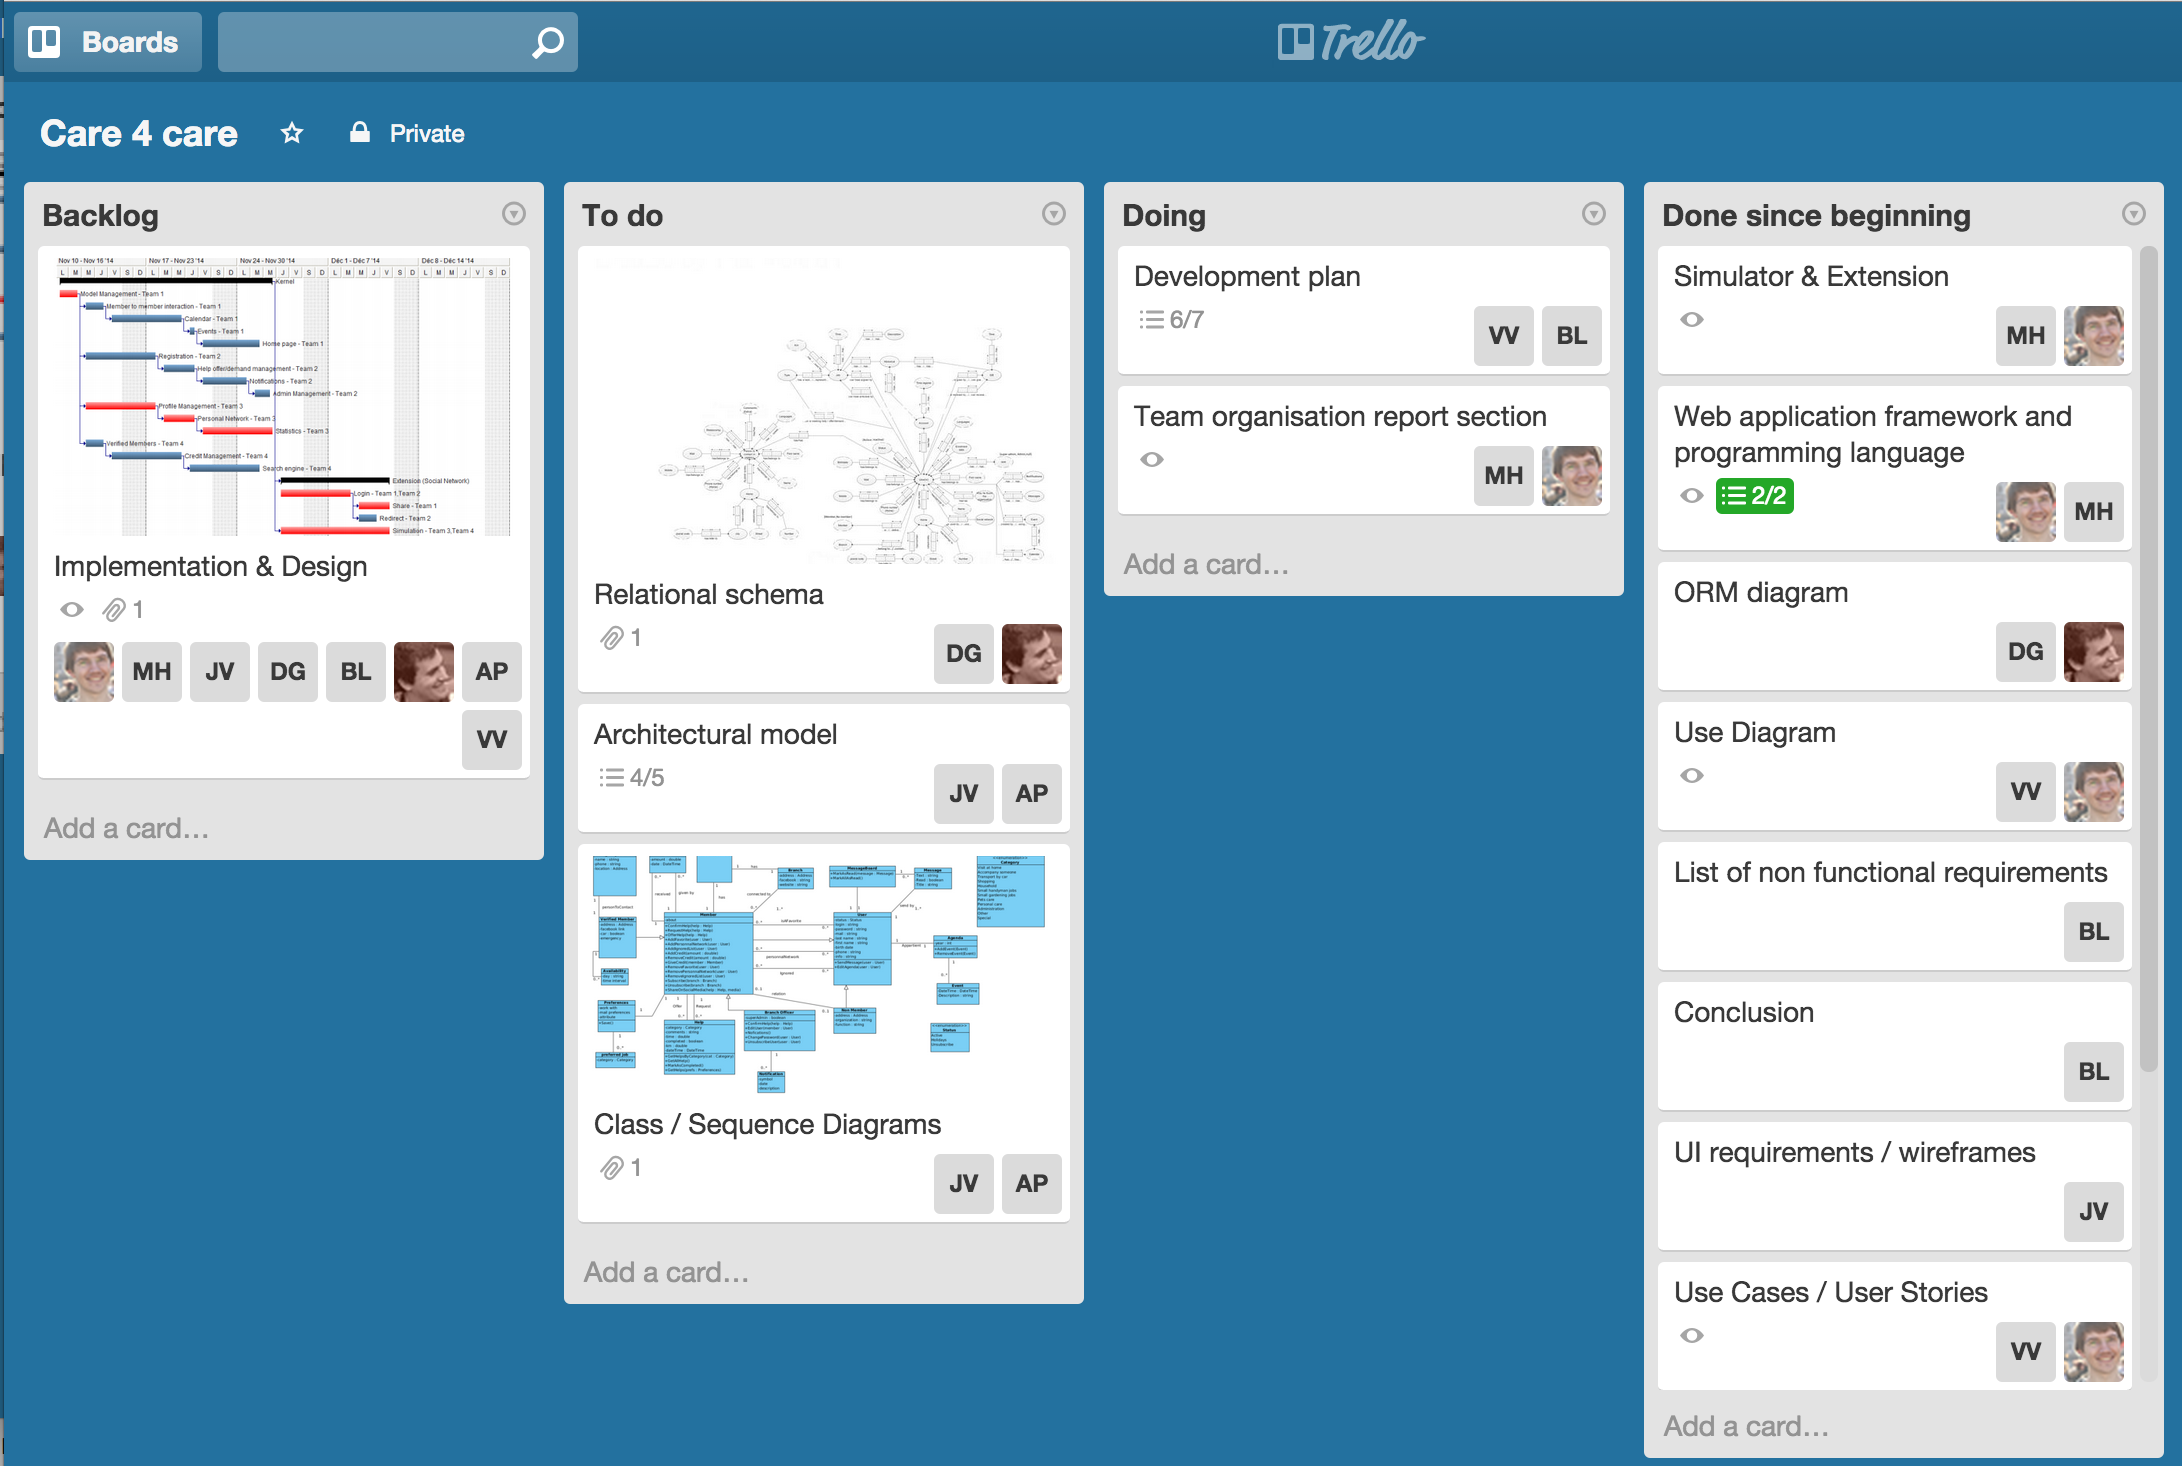
\includegraphics[width=\textwidth]{trello.png}
   \caption{\label{trello} Trello}
\end{figure}

Trello allows our team to organize the tasks scheduling.
We can create task and assign them to our members.
We are able to update each card and sort them by lists.
For the moment, as you can see on figure~\ref{trello}, we have four lists : \tit{Backlog}, \tit{To do}, \tit{Doing} and \tit{Done since beginning}.
This organization is really helpful because we can see the progression in a glance.

\subsection{Github}

\begin{figure}[!ht]
   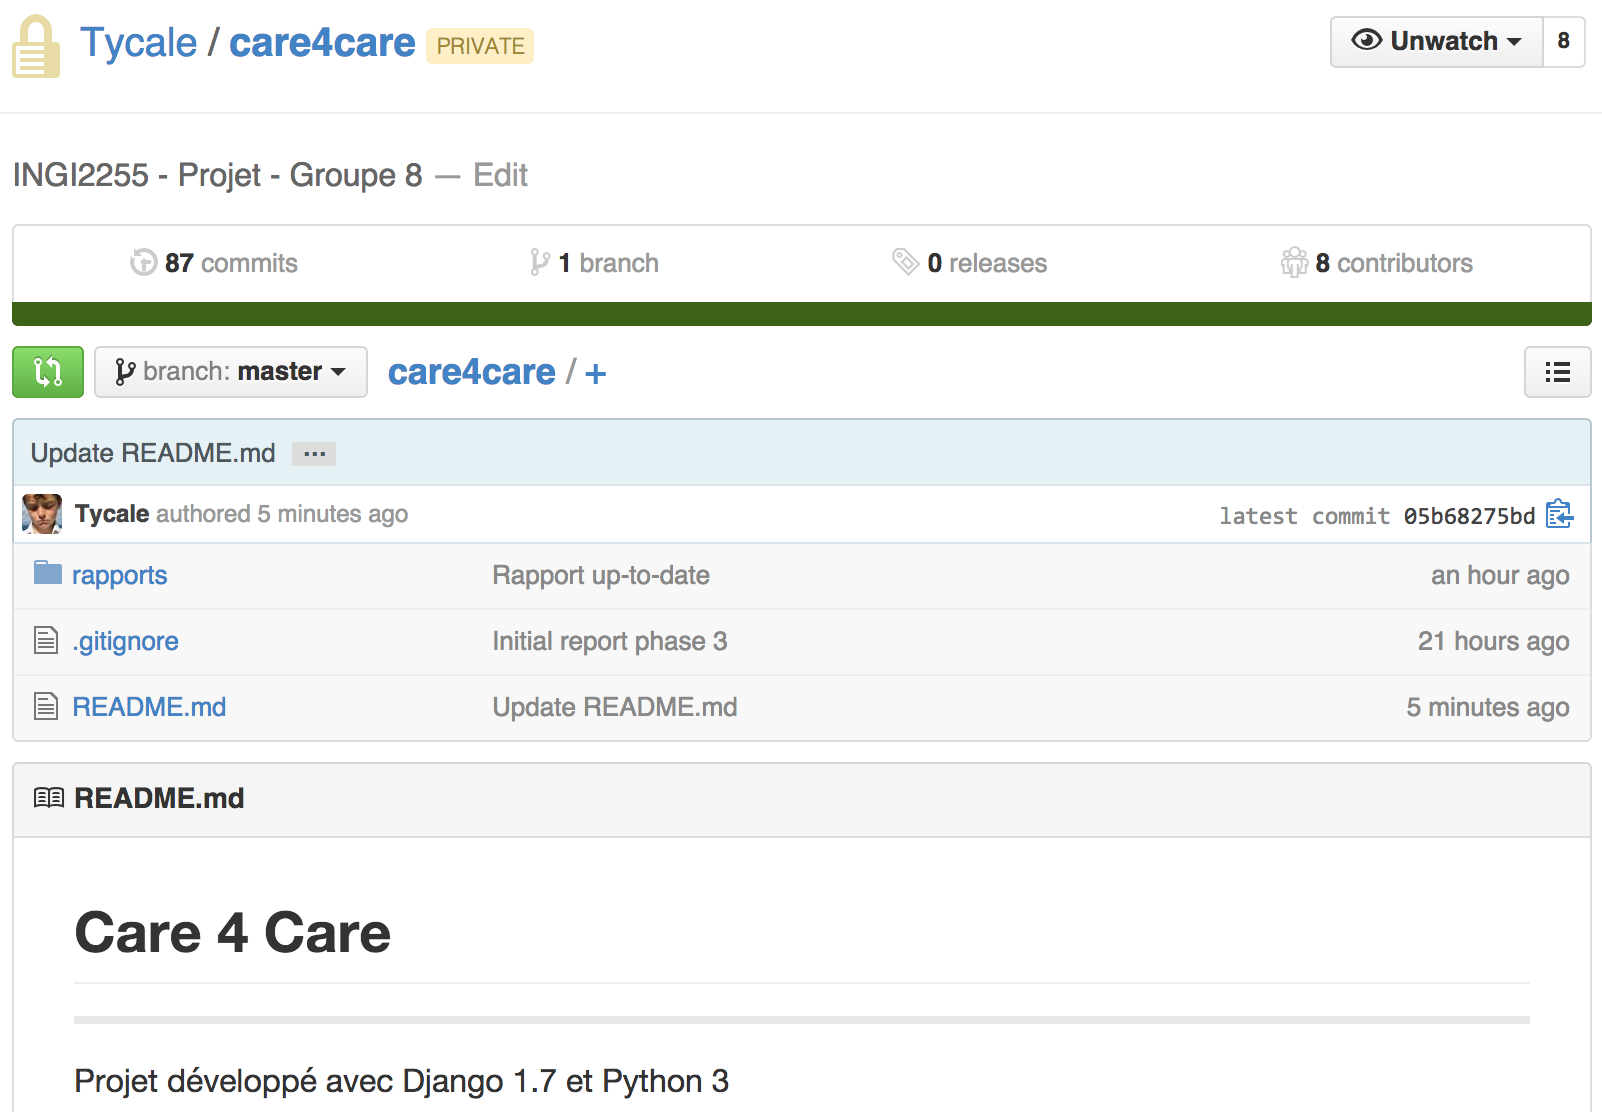
\includegraphics[width=\textwidth]{github.png}
   \caption{\label{github} github repository – care4care}
\end{figure}

Github is well-known in the developers community.
This platform permits us to synchronise the files and see the differences between versions.
We asked for a private repository thanks to the educational program.
The difference between two revisions is called a \enquote{commit}.
As shown in the figure~\ref{github}, you can see that we have 87 commits delivered by 8 contributors.

\subsection{Facebook}

\begin{figure}[!ht]
   \includegraphics[width=\textwidth, height=7cm]{leader.png}
   \caption{\label{facebook} Cover picture of our private group}
\end{figure}

We have a secret facebook with all members.
We use this platform to find dates to meet together and make announcements.
Our leader uses a \enquote{sticker} system to reward or to penalize our work. As you can see in the figure~\ref{facebook}, a \enquote{sun} means that you did something really good and a \enquote{cloud} means that you did something wrong.





\section{Data}
\subsection{Object-Role Modeling Schema}

%Schema ici

\subsection{Object-Relational Mapping}
Django uses an ORM (Object-Relational Mapping).
A ne pas confondre avec notre schéma ORM (object-relational mapping).
L'ORM de Django permet de nous libérer de la gestion de la base de donnée.
Django nous permet de créer des modèles (sous forme de classe) afin de définir nos données.

Imaginons que nous définissons un modèle \texttt{Person} dans notre application \texttt{members} du projet \texttt{care4care}.

\begin{lstlisting}[frame=single, caption=file care4care/members/models.py]  % Start your code-block
from django.db import models

class Person(models.Model):
    first_name = models.CharField(max_length=30)
    last_name = models.CharField(max_length=30)
\end{lstlisting}

Django va automatiquement créer une table dans la base de données en fonction de notre modèle que nous avons défini.
Ainsi, pour cet exemple, django va créer une table \texttt{members\_person} contenant nos deux champs : \texttt{first\_name} et \texttt{last\_name}.
Django supporte plusieurs base de données tel que sqlite, postgresql, mysql, etc.
En fonction du gestionnaire de base de donnée choisi, la requête que django va générer sera différente. 

Il est inutile de donner un \texttt{id} à nos modèles car django crée ce champ par défaut.

Si nous voulons récupérer tous les objets d'un modèle, nous pouvons simplement écrire : \lstinline{Person.objects.all()}.
Cet appel va créer une requête SQL pour nous afin de sélectionner tous les objets \texttt{Person} en DB.
L'objet retourné par ce type de requête est un \enquote{QuerySets}.
Nous pouvons appliquer des filtres aux \enquote{QuerySets} : \lstinline{Person.objects.filter(last_name__startswith='T')}.
Cette requête va sélectionner toutes les \texttt{Person} dont leur \texttt{last\_name} commence par \enquote{T}.
QuerySets are lazy – the act of creating a QuerySet doesn’t involve any database activity.





\subsection{Best practices}

To ensure that code and design are of good quality we have decided several things :


\begin{itemize}
\item Follow a coding guide to have readable code
\item Make code reviews
\item Use Unit Testing framework
\item Use existing library
\end{itemize} 

\subsubsection{Coding Style}
	
We will be using the \enquote{Style Guide for Python Code} from PEP 8 found on python.org because it is well knowed and widespread. 
The advantage of a coding guideline is that it improve the readability of code by us and most importantly by other developers. 
It also make the code consistent across an entire project developed by different peoples, avoid duplication of code and reduce bug-rate. 
 
Here is the main things we will try to be consistent with : 

\begin{itemize}
\item Indentation : 4 spaces per indentation level
\item Use snake case as naming style
\item Maximum Line Length of 79 characters
\item Separate top-level function and class definitions with two blank lines
\item Try to write comprehensive code
\item Comment your code if the code is not easy to understand
\item Source Code file use UTF-8 format
\item Imports on separate lines
\item Avoid extraneous whitespace
\item Avoid Global Variable
\end{itemize} 


\subsubsection{Code Reviews}
	
Each time a task will be finished or a bug will be resolve, the code will be review by someone else from the group. 
We hope that doing this will ensure well written code and avoid introducing new bugs when correcting one.  
 
This will be possible with the help of github and the pull requests functionality, we will also need a bug tracking tool like trello or a most advance one like Jira. Some member in the group have already experience with Jira and it is very useful to track bug and review code for a specific bug. 
 
Code reviews are also good for improving the code because multiple brains are usually better than one. 
 
\subsubsection{Unit Testing} 
 
Unit testing our application is a great way to detect bugs early in the development phase and gain some precious time. That is why we will use the Unit testing framework from python named \enquote{unittest} and also Selenium explained above (which also test the user interface). 
 
The unit tests will run frequently to detect bugs introduced by new code or modification of existing code. This way we hope members of the group will rarely commit code that breaks the application and not notice it. 
 
Unfortunately we do not have enough time to cover 100\% of our code with unit test so we will have to decided which are the most critical parts of our software. 
 
\subsubsection{Existing library} 
 
We will be carful about not reinventing the wheel and use already available code. The goal of this is to reduce development time and testing time.  
For example if a library is well know and already tested we do not have to do it ourselves. 
 
The django framework is already very good in that sense because many functionality of a web application are there.
 
\end{document}
